\documentclass[letterpaper]{article}

\usepackage{Bioconductor}
\usepackage{graphicx}
\usepackage{fullpage}
\title{\Bioconductor{} Annual Report (preliminary)}
\author{Lori Kern\\ Roswell Park Comprehensive Cancer Center}
\date{Nov 30, 2021}

\begin{document}

\maketitle

\tableofcontents

\section{Project Scope}

\Bioconductor{} provides access to software for the analysis and
comprehension of high throughput genomic data. Packages are written in
the \R{} programming language by members of the \Bioconductor{} team
and the international community. \Bioconductor{} was started in Fall,
2001 by Dr.\ Robert Gentleman and others, and now consists of 2083
software packages for the analysis of data ranging from single-cell
sequencing to flow cytometry.

The mission of the Bioconductor project is to develop, support, and disseminate
free open source software that facilitates rigorous and reproducible analysis of
data from current and emerging biological assays. We are dedicated to building a
diverse, collaborative, and welcoming community of developers and data
scientists.

\subsection{Funding}

Lori does not have information to summarize.

\subsection{Package and Annotation Resources}

\R{} software packages represent the primary product of the
\Bioconductor{} project. Packages are produced by the \Bioconductor{}
team and from international
contributors. Table~\ref{tbl:analysis_pkgs} summarizes growth in the
number of packages hosted by \Bioconductor{}, with
\href{https://bioconductor.org/packages/3.14}{2083 software packages}
available in release 3.14.  The project produces 901 `annotation'
packages to help researchers place analytic results into biological
context. Annotation packages are curated resources derived from
external data sources, and are updated at each release. The project
also produces 408 `experiment data' packages to provide heavily
curated results for pedagogic and comparative purposes. We have
standardized reproducible, cross-package protocols into 29 `workflow'
packages. There are also
\href{http://bioconductor.org/checkResults/3.14/books-LATEST/}{8 `books`} for
in-depth analysis mostly focused on Single Cell Analysis.


The project has developed, over the last several years, the
`AnnotationHub' and `ExperimentHub` resources for serving and managing
genome-scale annotation data, e.g., from the TCGA, NCBI, and
Ensembl. There are 60134 records in the AnnotationHub, and 6075
ExperimentHub records.

The number of distinct IP addresses downloading software continues to
grow in an approximately exponential fashion
(Figure~\ref{fig:download-stats}).

\begin{table}
  \begin{center}
    \caption{Number of contributed packages included in each
      \Bioconductor{} release.  Releases occur twice per year.}
    \label{tbl:analysis_pkgs}
    \begin{tabular}{llc|llc|llc|llc|llc}
      \\
      \multicolumn{2}{l}{Release} & N & 
      \multicolumn{2}{l}{Release} & N & 
      \multicolumn{2}{l}{Release} & N &
      \multicolumn{2}{l}{Release} & N \\\hline\noalign{\smallskip}
      2002 & 1.0 & 15    & 2006 & 1.8 & 172  & 2010 & 2.6 & 389 & 2014 & 2.14 & 824  & 2018 & 3.7  & 1560\\ 
           & 1.1 & 20    &      & 1.9 & 188  &      & 2.7 & 419 &      & 3.0  & 936  &      & 3.8  & 1649\\
      2003 & 1.2 & 30    & 2007 & 2.0 & 214  & 2011 & 2.8 & 467 & 2015 & 3.1  & 1024 & 2019 & 3.9  & 1741\\
           & 1.3 & 49    &      & 2.1 & 233  &      & 2.9 & 517 &      & 3.2  & 1104 &      & 3.10 & 1823\\
      2004 & 1.4 & 81    & 2008 & 2.2 & 260  & 2012 & 2.10 & 554& 2016 & 3.3  & 1211 & 2020 & 3.11 & 1903\\
           & 1.5 & 100   &      & 2.3 & 294  &      & 2.11 & 610&      & 3.4  & 1294 &      & 3.12 & 1974\\
      2005 & 1.6 & 123   & 2009 & 2.4 & 320  & 2013 & 2.12 & 671& 2017 & 3.5  & 1381 & 2021 & 3.13 & 2042\\
           & 1.7 & 141   &      & 2.5 & 352  &      & 2.13 & 749&      & 3.6  & 1473 &      & 3.14 & 2083\\
    \end{tabular}
  \end{center}
\end{table}

\begin{figure}
  \begin{center}
    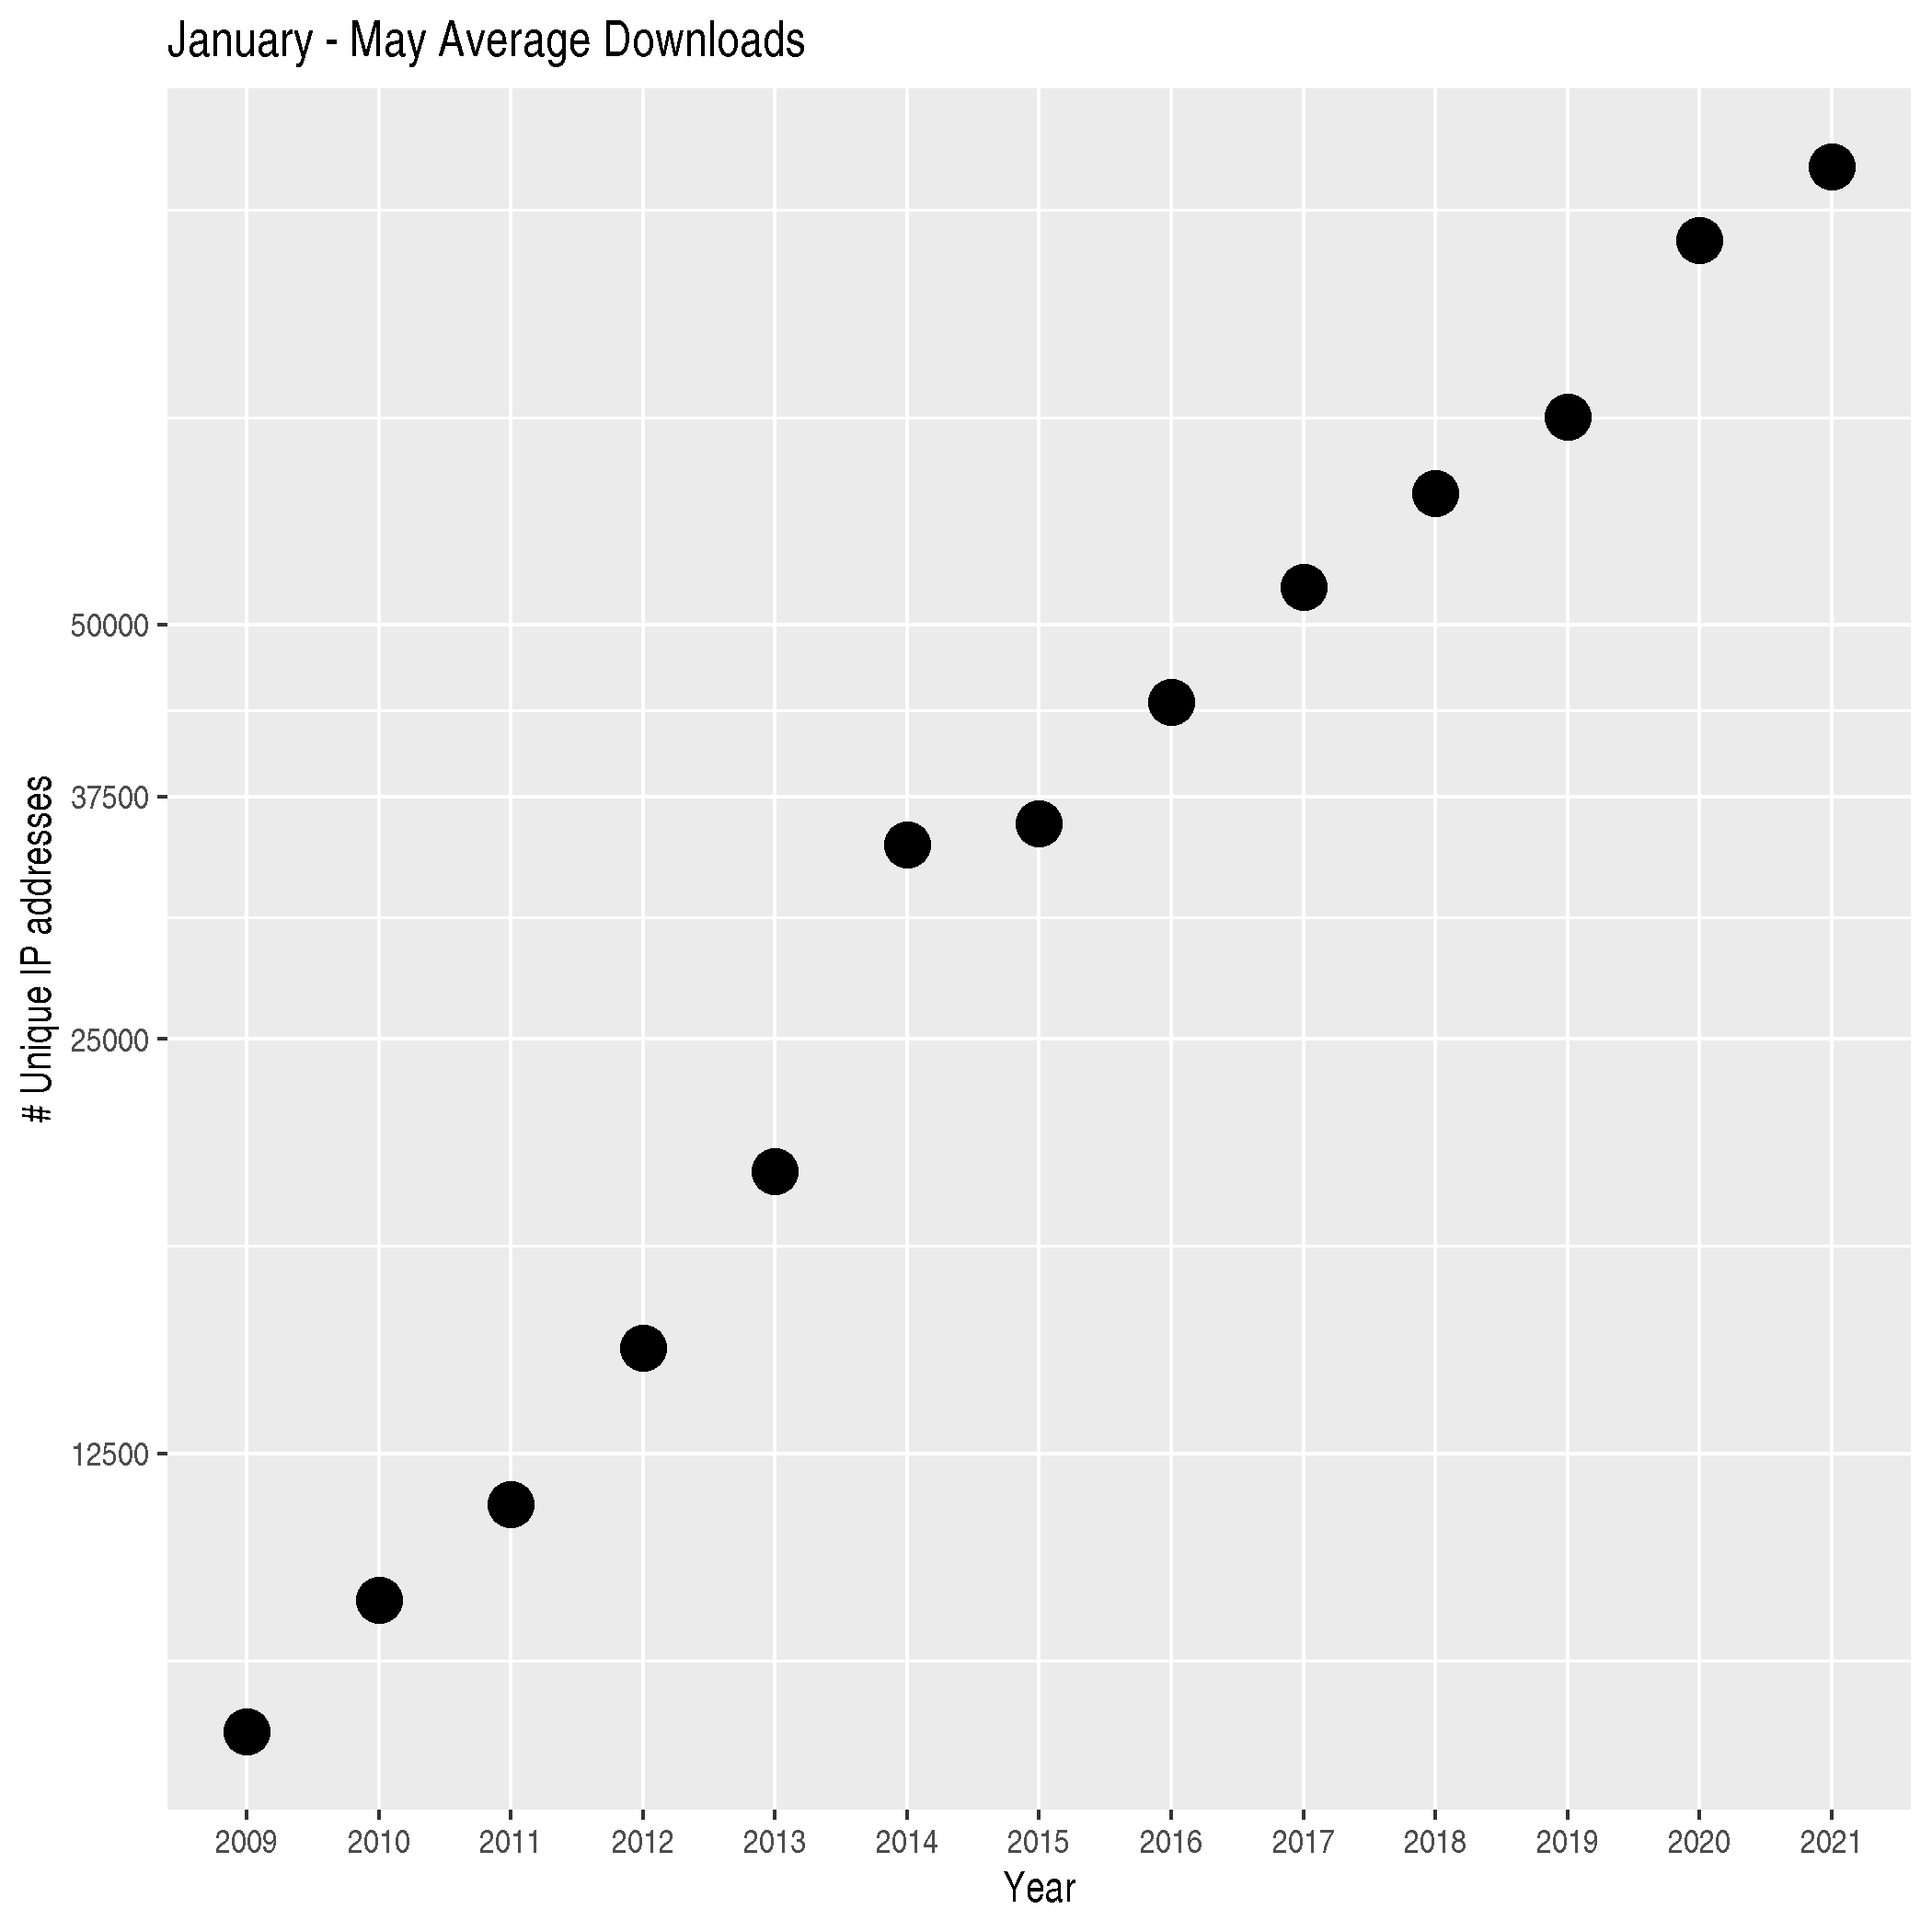
\includegraphics[width=.5\textwidth,height=!]{download-stats-2021}
    \caption{\Bioconductor{} package download statistics, average number
      of unique downloads, first six months of each year.}
    \label{fig:download-stats}
  \end{center}
\end{figure}


\subsection{Courses and Conferences}

Our annual conferences include:

\begin{itemize}
\item \href{https://bioc2020.bioconductor.org}{BioC2020}
  pivoted to a 5-day virtual conference, with reduced registration
  fee and participation reaching our maximum capacity of 500
  attendees. \href{https://bioc2021.bioconductor.org}{BioC2021} North American
  conference was held as a 3-day virtual conference from August 4-6; no in
  person components due to continued covid 2019 restrictions. Participation
  reached 809 attendees.    
\item \href{https://biocasia2021.bioconductor.org/}{BioCAsia2021}, held
  as a virtual conference from November 1-4, 2021. Talks were multilingual
  translating to Japanese, Mandarin, and English. There were estimated 430
  attendees.
\item \href{https://eurobioc2022.bioconductor.org/}{European
  Bioconductor Meeting}, was postponed to March 16-18, 2022 and currently is
  planned to be in person in Heidelberg, Germany.
\item \href{https://comunidadbioinfo.github.io/post/cdsb2020-building-workflows-with-rstudio-and-scrnaseq-with-bioconductor/#.YaY3DrtOnmF}{CDSB 2020 (Mexican Bioinformatics Encounter)} took place August 3-7, 2020 as a
  virtual workshop.
\item Bioconductor workshops were also held as virtual workshops in conjunction
  with \href{https://h3africa.org/}{H3Africa}
\end{itemize}


The \href{https://bioconductor.org/help/course-materials/}{course
  materials} section of the web site summarizes material from these
and some of the many other courses and conferences offered by
\Bioconductor and the \href{https://bioconductor.org/help/events/}{events
  calendar} list conferences, workshops, and other events that involve
\Bioconductor.



\subsection{Community Support}

The \Bioconductor{} \href{https://support.bioconductor.org}{support
  site} is used for help, announcements, and outreach worldwide. From January
01, 2021 to November 30, 2021, there are 2400 new users, 1901 `top-level` posts,
and 4933 comments (answers+comments). 

The support site was upgraded and standardized to be consistent with the
Biostars code base. Natay Aberra from Biostars has been instrumental in the
transition; Lori Kern from the core team is working with Natay to be able to
update and troubleshoot as necessary. 


Another form of communication for the Bioconductor community is the \Bioconductor{}
\href{https://community-bioc.slack.com}{community slack}. As of November 30,
2021, there are 1615 members of the community slack channel with 97 different channels.


We continue to provide the
\href{http://www.stat.math.ethz.ch/mailman/listinfo/bioc-devel}{bioc-devel},
mailing list forum for package contributors' questions and discussion
relating to the development of \Bioconductor{} packages. There are
1811 subscribers on this list. Table~\ref{tbl:av_posts} lists the number of
posts and number of unique authors per month as a monthly average since
2002. Recent increase in activity is likely due to (1) enforced requirement that
new package maintainers subscribe to the mailing list, and (b) using
the bioc-devel mailing list as a support forum for use of
git.bioconductor.org. 

\begin{table}
\begin{center}
\caption{Monthly average number of posts and number of unique authors
  for the \Bioconductor{} 'devel' mail list from January, 2005. 2021 does not
  include December information}
\label{tbl:av_posts}
\begin{tabular}{lcc|lcc|lcc}
  \\
       & Posts     & Authors   &      & Posts     & Authors   &      & Posts     & Authors\\
  Year & per month & per month & Year & per month & per month & Year & per month & per month\\
  \hline\noalign{\smallskip}
  2005 & 27        & 13        & 2011 & 52        & 24        & 2017 & 186 & 45 \\
  2006 & 39        & 19        & 2012 & 75        & 25        & 2018 & 160 & 48 \\
  2007 & 50        & 23        & 2013 & 97        & 34        & 2019 & 123 & 44 \\
  2008 & 27        & 18        & 2014 & 139       & 41        & 2020 & 134 & 47 \\
  2009 & 26        & 17        & 2015 & 142       & 43        & 2021 & 104 & 38 \\
  2010 & 30        & 18        & 2016 & 153       & 45\\
\end{tabular}
\end{center}
\end{table}


Web site summary get from google analytics?


\textbf{Lori Did Not Update Anything below this section}



\subsection{Publication}

\Bioconductor{} has become a vital software platform for the worldwide
genomic research community, with more than 38,500 PubMedCentral
full-text citations for `Bioconductor'. Table~\ref{table:pubMed}
summarizes PubMed author / title / abstract or PubMedCentral full-text
citations since 2003.

\begin{table}
  \caption{PubMed title and abstract or (2012 and later) PubMedCentral full text searches for ``Bioconductor'' on
    publications from January, 2003 -- July, 2020.}
  \label{table:pubMed}
  \begin{center}
    \begin{tabular}{rc|rc|rc|rc|rc}
      Year &  N & Year &  N & Year &    N & Year  & N    & Year  & N\\\hline\noalign{\smallskip}
      2003 &  7 & 2007 & 44 & 2011 &   68 & 2015  & 3138 & 2019  & 5939 \\
      2004 & 13 & 2008 & 52 & 2012 & 1386 & 2016  & 3415 & 2020* & 3224*\\
      2005 & 19 & 2009 & 62 & 2013 & 2048 & 2017  & 3988 & \\
      2006 & 30 & 2010 & 52 & 2014 & 2401 & 2018  & 4610 & \\
    \end{tabular}
  \end{center}
\end{table}

\href{https://bioconductor.org/help/publications/}{Featured and recent
  publications} citing \Bioconductor{} are available on the
\Bioconductor{} web site, and are updated daily. 

\section{New and Ongoing Accomplishments}

\subsection{Leadership structure \& community engagement}

The Technical Advisory Board (membership enumerated below) meets
monthly to discuss technical issues important to establishing and
maintaining project momentum. Over the past two years the structure
has been formalized with a governance document and procedures to
ensure influx of new participants through a public nomination process
followed by election to a three year term. The July, 2020 meeting saw
the departure of long-term board members Sean Davis and Michael
Lawrence, and Matt Ritchie's transition to co-leadership of the
newly-formed Community Advisory Board. New members include
Drs.\ Michael Love (UNC Chapel Hill), Hector Corrada Bravo
(Genentech), and Shila Ghazanfar (Cancer Research UK,
Cambridge). Martin Morgan departed as chair of the executive, with
Vincent Carey taking that role (previously, vice-chair), Levi Waldron
becoming vice-chair (previously secretary), and Charlotte Soneson
becoming secretary.

The Community Advisory Board was established this year to more
directly address the training and outreach mission of
\Bioconductor. Motivation is several-fold. It is clear the project as
a whole would benefit from attention focused on community
engagement. The combined purview of the technical and community boards
is too large for a single board. The second board expands leadership
opportunities within the project.

The Community and Technical boards, and the overall leadership
structure of the project remains a work-in-progress. There is a need
for established lines of communication and coordination between
boards, as well as a clear organizational plan describing the
relationship between them. Technical activities of the board can be
supported by grant funding, particularly though not exclusively to
support the core team, whereas activities of the community board may
both generate revenue (e.g., from conferences) and expenditures in
ways that are less consistent with current funding sources. The
Bioconductor Foundation of NA may represent one mechanism for managing
these financial resources, but this implies greater integration of the
Foundation into the overall organization structure.

\subsection{Containers and clouds}

Involvement with the AnVIL project has helped to clarify container and
cloud based strategies for \Bioconductor, resulting in several
interesting developments.

We have revised our docker strategy to provide images with necessary
system dependencies, rather than pre-installed packages. This provides
a flexible image that can be easily tailored to the diverse needs of
our community. The images are built on community-standard 'rocker'
base images. One consequence of a docker image is that fixed
underlying system requirements allow Linux-based 'binary' package
installation. Binary installations are much faster than source
installations, allowing containers to be used effectively for tasks
with relatively short life cycles, e.g., during teaching, running
workflows, etc. We have explored binary \Bioconductor{} package
repositories within AnVIL, and have to some extent had binary images
thrust upon us by the adoption of the RStudio CRAN package manager by
the underlying rocker container; there have been important lessons
learned about providing robust and stable containers, including the
need for much more extensive integration tests of our own containers.

Our involvement with the AnVIL project has provided opportunities to
use our container knowledge to explore cloud-based computation. Again
there are several insights from this, although the situation seems one
more of promise that delivery at the moment. Access to large data
resources, including data requiring authenticated access and to
scalable computing capabilities seems very promising. The use of
containers as a mechanism for delivering \R{} / \Bioconductor{},
including \emph{RStudio}, moves the burden of 'system administration' from
the user to the \Bioconductor{} core team. Cost-management and the
need to fund use through Google and credit card introduces many
barriers to use by the \Bioconductor{} community. Workshop
infrastructure developed by Sean Davis for our just-concluded annual
conference illustrates opportunities for scalability through the use
of clouds and containers, with thousands of workshops launched with
minimal end-user complaint and modest cost using Google Kubernettes
Engine.

\subsection{Software}

\begin{description}
  \item[\Biocpkg{BiocIO}] extracts from the \Biocpkg{rtracklayer}
    package a common language and flexible infrastructure for
    importing and exporting file types, simplifying file access and
    focusing development efforts on more advanced file processing
    models.
\item[\Biocpkg{GenomicRanges}] and friends represent a mature infrastructure for
  working with range-based and sequence data.
\item[\Biocpkg{DelayedArray}] and the \Biocpkg{HDF5Array} back-end
  provide a framework for managing large out-of-memory rectangular
  data representations.
\item[\Biocpkg{BiocFileCache}] manages a cache of local or remote files.
\item[\Biocpkg{AnnotationHub}] and \Biocpkg{ExperimentHub} and
  supporting infrastructure play increasingly important roles in
  distribution of annotation and experiment results.
\item[Incremental enhancements] to \Biocpkg{BiocParallel},
  \Biocpkg{GenomicFiles}, \Biocpkg{BiocCheck},
  \Biocpkg{MultiAssayExperiment}, \Biocpkg{SummarizedExperiment} and
  other core packages.
\end{description}

\subsection{Infrastructure}

\begin{description}
\item[Version control] We continue to use package-specific git
  repositories hosted at git.bioconductor.org for package
  maintenance.

  Some aspects of the use of git.bioconductor.org, especially access
  management, represent pain points (as evidenced by frequent reports
  of difficulties on the bioc-devel mailing list) where further effort
  is needed to smooth the experience.
\item[New package contributions] use
  \href{https://github.com/Bioconductor/Contributions}{Github} and a
  public review process. The process has been updated so that new
  maintainers become familiar with use of the \Bioconductor{} git
  repository during the package ingestion process. Effort expended on
  reviewing packages is considerable; generally, the review process
  has become both more protracted and less comprehensive in response
  to this.
\item[Single package builder] (SPB) is used to build packages in the
  review process on commit. Builds occur across Linux, macOS, and
  Windows environments that closely resemble the \Bioconductor{} build
  system, providing developers with immediate feedback for iterative
  improvement of their packages. The SPB has been updated to use
  git.bioconductor.org as a repository source. This was done so that
  new package contributes use the \Bioconductor{} git repository
  during the review process (see previous point). An easy technical
  extension is to allow build-on-commit for existing as well as new
  packages; this would provide a build experience, complementary to
  the nightly builds, that is more comparable to the continuous
  integration systems many of our developers are familiar with. A
  necessary step before implementing this is to understand whether a
  build-on-commit system would be too taxing to the physical resources
  of the build system.
\end{description}

\subsection{User Support}

\begin{description}
\item[\href{https://support.bioconductor.org}{Support site}] has
  established itself as an important resource. We have been engaged in
  an extended collaboration with Biostars author to harmonize our code
  base with upstream code, to enhance security, and to prepare for the
  release of an updated support forum.
\item[\href{https://bioconductor.org/help/workflows}{Workflows}]
  provide cross-package training material and integrate with the
  \href{http://f1000research.com/channels/bioconductor}{F1000
    \Bioconductor{} channel}. Workflows are now distributed as
  standard \R{} packages built regularly, distributed through
  CRAN-style repositories, and organized on the web site using the
  same approach as other package types.
\item[\href{https://community-bioc.slack.com}{Slack}] channels for the
  core team and \Bioconductor{} community are providing new avenues
  for communication. The community slack channel was an important
  catalyst in the HCA grantsmanship process, and in several
  significant collaborative software initiatives lead by community
  members.

  Use of slack within the community poses several challenges. Support
  channels have become fragmented, with users and developers posting
  requests to the support site, developer mailing list, specific
  issues on github repositories, and slack. Even with a substantial
  discount, the slack channel is increasingly expensive. The large
  number of channels, and the opportunity for private messaging, poses
  challenges for ensuring community code of conduct and appropriate
  use.
\item[\href{https://bioconductor.org/help/course-materials}{Course
    Materials}] organize and make accessible recent course and
  training material.
\end{description}

\section{Core Tasks \& Capabilities}

\subsection{Core Tasks}

\begin{enumerate}

\item Package Building and Testing.  The \Bioconductor{} project
  provides access to its packages through repositories hosted at
  \texttt{bioconductor.org}.  One of the services provided to the
  \Bioconductor{} community is nightly automated build and check of
  all packages.  Maintaining the automated build and test suite and
  keeping the published package repositories updated requires a
  significant amount of time on the part of the Roswell
  \Bioconductor{} team.  As the project has grown, the organizational
  and computational resources required to sustain the package build
  system have also increased; see section~\ref{sec:pkg_building}.

\item Package dissemination via
  \href{https://bioconductor.org}{https://bioconductor.org} and
  underlying CRAN-style repository using Amazon CloudFront for global
  distribution.

\item Software development.

\item End-user support via
  \href{https://support.bioconductor.org}{https://support.bioconductor.org}
  and the bioc-community slack channel.

\item Developer support via the
  \href{https://stat.ethz.ch/mailman/listinfo/bioc-devel}{bioc-devel}
  mailing list.

\item New package submission.  The \Bioconductor{} project relies on
  technical review process of candidate packages to ensure they
  contain high-quality software.

\item Annotation data packages.  The \Bioconductor{} project
  synthesizes genomic and proteomic information available in public
  data repositories in order to annotate genomic sequences and probes
  of standard microarray chips.  These annotation data packages are
  made available to the community and allow \Bioconductor{} users to
  easily access meta data relating to their experimental platform.  We
  maintain automated tools to parse the available information.

\item Semi-annual releases, typically in March and October.

\end{enumerate}

\subsection{Hardware and Infrastructure}
\label{sec:pkg_building}

The \Bioconductor{} project provides packages for computing platforms
common in the informatic community.  We provide source packages
that can be installed on Linux and most UNIX-like variants, as well as
binary packages for Windows and macOS.  To ensure that packages are
consistently documented, easy to install, and functioning properly, we
run a nightly build during which we test all packages in the release
and development repositories.  

The build system currently consists of at least two Windows machines,
two Linux machines, and two macOS machines. The Windows, Linux, and
one macOS machines are physical servers located at Roswell Park, the
remaining macOS machine is rented via MacStatdium. The web site,
support site, AnnotationHub, and additional servers are hosted on
virtual machines, some of which are Amazon machine instances. The
build machines are recently updated, with adequate room for growth.

\subsection{Key Personnel}
\label{sec:key_personnel}

The \textbf{Core Development Team} are primarily employees of Roswell
Park Cancer Institute, developing software and other infrastructure
and ensuring day-to-day operation of the project. Core team members in
the period covered by this report include Martin Morgan, Herv\'{e}
Pag\`{e}s, Marcel Ramos, Lori Shepherd, Nitesh Turaga, Daniel van
Twisk, and Kayla Interdonato. The core team is stable but in chronic
need of additional members.

The \textbf{Technical Advisory Board} provides guidance through
monthly telephone conference calls. Current members include: Vince
Carey, Brigham \& Women’s, Harvard Medical School, USA. Chair; Levi
Waldron CUNY School of Public Health at Hunter College, New York, NY,
Vice-Chair; Charlotte Soneson, Friedrich Miescher Institute, Basel,
Switzerland, Secretary; Aedin Culhane, Dana-Farber Cancer Institute,
Harvard School of Public Health, USA; Hector Corrada Bravo, Genentech
Research and Early Development, USA; Laurent Gatto Institut de Duve,
Belgium; Robert Gentleman, Computational Biology, 23andMe, USA; Shila
Ghazanfar, Cancer Research UK, Cambridge; Kasper Daniel Hansen,
Bloomberg School of Public Health, Johns Hopkins University; Stephanie
Hicks Department of Biostatistics, Johns Hopkins Bloomberg School of
Public Health, USA; Wolfgang Huber European Molecular Biology
Laboratory, Heidelberg, Germany; Rafael Irizarry Dana-Farber Cancer
Institute, USA; Aaron Lun, Genentech Research and Early Development,
USA; Michael Love, University of North Carolina-Chapel Hill, USA;
Martin Morgan, Roswell Park Comprehensive Cancer Center, Buffalo, NY,
USA.

The recently formulated \textbf{Community Advisory Board} supports the
\Bioconductor{} mission by empowering user and developer communities
by coordinating training and outreach activities, and enabling
productive and respectful participation by Bioconductor users and
developers at all levels of experience. Current members include:
Yagoub Adam, Covenant University, Nigeria; Benilton Carvalho,
University of Campinas, Brazil; Leonardo Collado-Torres, Lieber
Institute for Brain Development, USA; Aedin Culhane, Dana-Farber
Cancer Institute, USA; Saskia Freytag, Harry Perkins Institute of
Medical Research, Australia; Susan Holmes, Stanford, USA; Kozo
Nishida, RIKEN Center for Biosystems Dynamics Research, Japan;
Johannes Rainer, Eurac Research, Italy Matt Ritchie, The Walter and
Eliza Hall Institute of Medical Research, Australia; Lori Shepherd,
Roswell Park Comprehensive Cancer Center, USA.

The \textbf{Scientific Advisory Board} provides oversight through
yearly meetings. Current members include: Robert Gentleman (Advisory
Board Chair, 23andMe); Jenny Bryan (RStudio); Vincent Carey (Brigham
\& Women’s); Valentina di Francesco (NHGRI); Wolfgang Huber (European
Molecular Biology Laboratory); Rafael Irizarry (Dana Farber); Audrey
Kauffmann (Novartis); Martin Morgan (Roswell Park); Benjamin Neale
(Broad Institute); Michael Schatz (Johns Hopkins University); Jay
Shendure (University of Washington); Levi Waldron (CUNY School of
Public Health). Audrey Kauffman and Jay Shendure are new board members
starting a three-year term; Jan Vitek leaves the board after three
years of service, for which we are grateful. Michael Schatz has
graciously agreed to complete James Taylor's term.

\end{document}
